
For each kid $k$, $f_{tone}^k$ moves with the atmospheric load according to

\begin{equation}
f_{tone}^k = C_0^k + C_1^k T_{atm}[1-e^{-\tau/\sin\delta}]
\end{equation}

where $\delta$ is the elevation. The {\tt skydip} procedure consists in moving
the telescope in elevation step by step and to monitor, for each kid, the
evolution of $f_{tone}^k$ vs the air mass and to fit the opacity $\tau$ and
$C_0^k$ and $C_1^k$. All the skydips (that were obtained under various opacity
conditions) are analysed together to break the degeneracies between these
parameters. The procedure has two steps. First, all the skydips are analysed
individually to simply measure $f_{tone}^k$ for each stable elevation and fit
simultaneously all the parameters. Error bars on $\tau$ are estimated by doing
this procedure on blocks of 40 kids only and getting a dispersion on the
resulting $\tau$ from the different blocks. Usually the dispersion comes out as
$4\times 10^{-3}$ at 1mm and $1\times 10^{-3}$ at 2mm. Once the $\tau$ values
are estimated for each skydip (as the average over the blocks), we compute
(while fixing $\tau$) the $C_0$ and $C_1$ final values for each kid. We thus
retrieve the coefficients of all the Kids even though some of them could not
contribute to the tau determination.

%% \begin{figure}
%% \begin{center}
%% 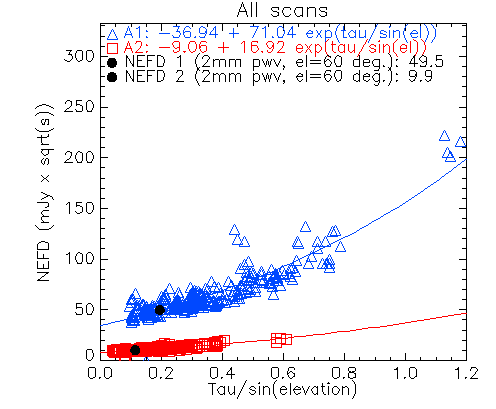
\includegraphics[clip, angle=0, scale =
%%   0.5]{Figures/NEFD_vs_tau_20170226s415_FXDC0C1_Jy_common_mode_kids_out.png}
%% 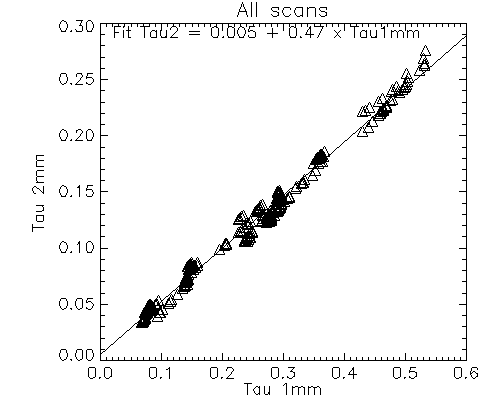
\includegraphics[clip, angle=0, scale =
%%   0.5]{Figures/tau1_tau2_20170226s415_FXDC0C1_GaussPhot_common_mode_kids_out.png}
%% \caption{}
%% \label{fig:fov}
%% \end{center}
%% \end{figure}

\begin{figure}
\begin{center}
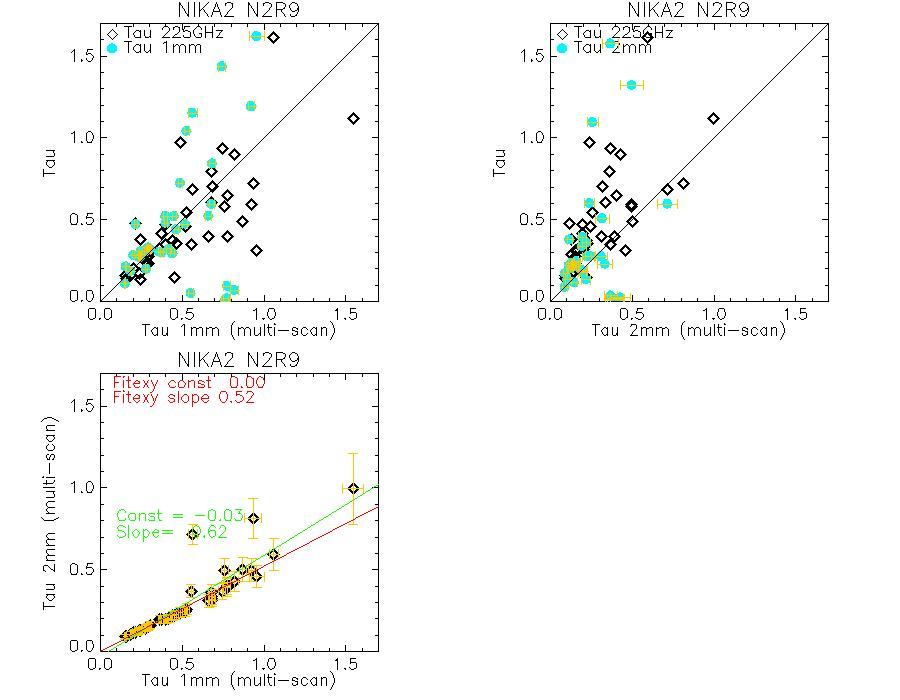
\includegraphics[clip, angle=0, scale = 0.5]{Figures/test_allskd_N2R9.jpg}
\caption{{\bf Fix me : improve plot quality and plot only the 3rd one.}}
\label{fig:test_allskd_N2R9}
\end{center}
\end{figure}
